% Finite-Time Convergence Illustration
% TikZ diagram for Chapter 4 - STA convergence proof

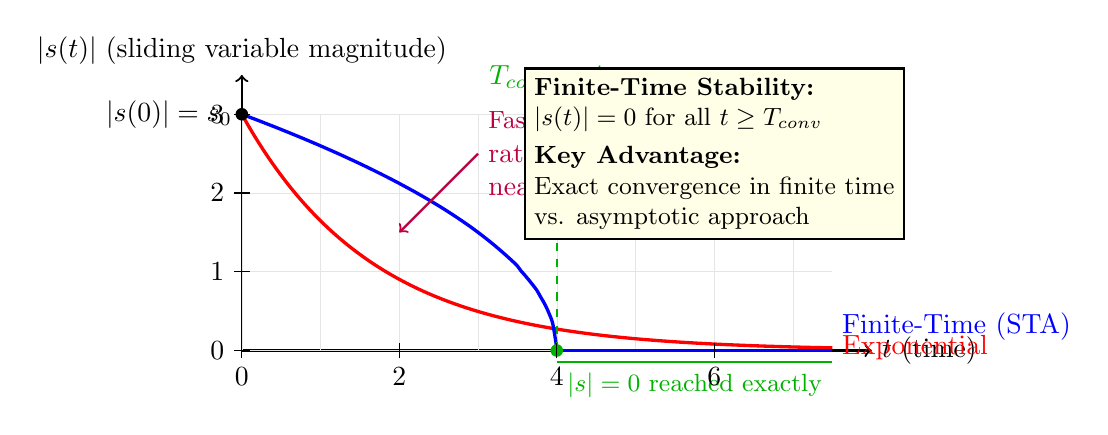
\begin{tikzpicture}[scale=1.0]

    % Axes
    \draw[->, thick] (0, 0) -- (8, 0) node[right] {$t$ (time)};
    \draw[->, thick] (0, 0) -- (0, 3.5) node[above] {$|s(t)|$ (sliding variable magnitude)};

    % Grid
    \draw[gray!20, very thin] (0, 0) grid (7.5, 3);

    % Asymptotic convergence (Classical SMC / Exponential)
    \draw[red, very thick, samples=80, smooth, domain=0:7.5]
        plot ({\x}, {3*exp(-0.6*\x)});
    \node[red, right] at (7.5, {3*exp(-4.5)}) {Exponential};
    \node[red, align=center] at (5, 2.5) {\small Asymptotic:\\$t \to \infty$};

    % Finite-time convergence (STA)
    \draw[blue, very thick, samples=80, smooth, domain=0:4]
        plot ({\x}, {3*pow((1 - \x/4), 0.5)});
    \draw[blue, very thick] (4, 0) -- (7.5, 0);
    \node[blue, right] at (7.5, 0.3) {Finite-Time (STA)};

    % Convergence time marker
    \draw[dashed, green!70!black, thick] (4, 0) -- (4, 3);
    \node[green!70!black, above] at (4, 3.2) {$T_{\text{conv}} = 4$ s};
    \fill[green!70!black] (4, 0) circle (0.08);

    % Zero line emphasis
    \draw[thick, green!70!black] (4, -0.15) -- (7.5, -0.15) node[midway, below] {\small $|s| = 0$ reached exactly};

    % Initial condition
    \fill[black] (0, 3) circle (0.08) node[left] {$|s(0)| = s_0$};

    % Convergence rate annotation
    \draw[<-, thick, purple] (2, 1.5) -- (3, 2.5)
        node[right, align=left] {\small Faster convergence\\rate than exponential\\near $s = 0$};

    % Comparison box
    \node[draw, thick, fill=yellow!10, align=left, font=\small] at (6, 2.5) {
        \textbf{Finite-Time Stability:}\\
        $|s(t)| = 0$ for all $t \geq T_{\text{conv}}$\\[0.1cm]
        \textbf{Key Advantage:}\\
        Exact convergence in finite time\\
        vs. asymptotic approach
    };

    % Tick marks
    \foreach \x in {0, 2, 4, 6}
        \draw (\x, -0.1) -- (\x, 0.1) node[below, yshift=-2mm] {$\x$};
    \foreach \y in {0, 1, 2, 3}
        \draw (-0.1, \y) -- (0.1, \y) node[left, xshift=-2mm] {$\y$};

\end{tikzpicture}
